
%!TEX ROOT=ctutest.tex

\chapter{Rešerše}


\section{Podlahové topení}
U podlahového vytápění dochází k přenosu tepla do vytápěného prostoru převážně sáláním. Což má za následek, že se od sálající plochy ohřívají plochy osálané a teprve od sálajících a osálaných ploch se ohřívá okolní vzduch (druhá konvenkční složka z celkového tepelného toku). Naproti tomu při přenosu tepla pomocí tradičních radiátorů dochází k přenosu pomocí proudění (konvekční složka). Při podlahovém vytápění, teplo postupuje rovnoměrně, plošně a plynule od spodu místnosti, \ref{fig:rozlozeni-teplot-podlahove-vytapeni}. Zatímco radiátory ohřívají prostor z jednoho místa a rozložení teplot v místnosti je nerovnoměrné, \ref{fig:rozlozeni-teplot-radiatory}.

\begin{figure}[h]
     \centering
     \begin{subfigure}[b]{0.45\textwidth}
         \centering
         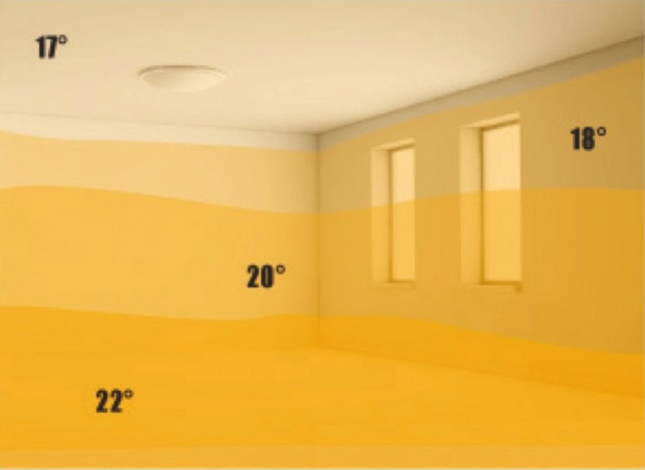
\includegraphics[width=\textwidth]{images/rozlozeni-teplot-podlahove-vytapeni.png}
         \caption{Rozložení teplot při použití podlahové topení.}
         \label{fig:rozlozeni-teplot-podlahove-vytapeni}
     \end{subfigure}
     \hfill
     \begin{subfigure}[b]{0.45\textwidth}
         \centering
         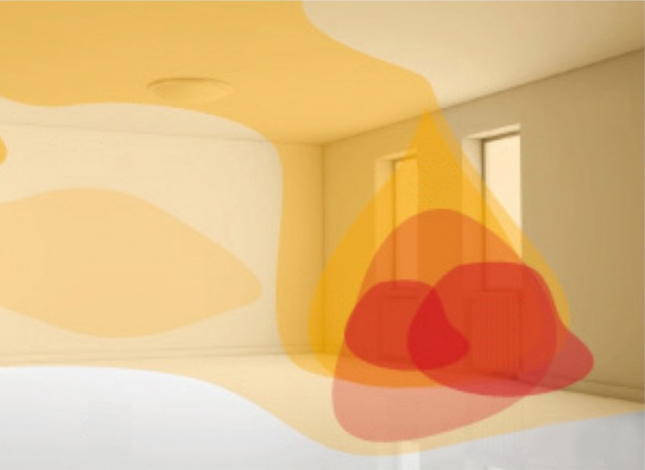
\includegraphics[width=\textwidth]{images/rozlozeni-teplot-radiatory.png}
         \caption{Rozložení teplot při použití radiátorů.}
         \label{fig:rozlozeni-teplot-radiatory}
     \end{subfigure}
\caption{Porovnání rozložení teplot při použití podlahové topení a radiátorů.}
\label{fig:porovnani-rozlozeni-teplot}
\end{figure}

\section{Zónová regulace vytápění}

\subsection{Principy zónové regulace}

\subsection{Dostupné komerční/nekomerční řešení zónové regulace podlahového vytápění}








